\chapter{Ideen und Konzepte}


% Hier geht es um die Fragestellung, wie Sie die formulierten Ziele der Arbeit erreichen wollen.
% Sie halten z.B. erste, grobe Ideen, skizzenhafte Lösungsansätze fest. Gibt es mehrere Wege, Ansätze
% um dieses Ziel zu erreichen, begründen Sie hier, warum Sie einen bestimmten Weg einschlagen.
% Beispiel für ein Softwareprojekt: Erste Gedanken über eine grobe Systemarchitektur. Ist z.B. eine
% Microservice-Architektur angebracht? Welche Alternativen bestehen, wo gibt es Problempunkte? Die
% Umsetzung, die Beurteilung der Machbarkeit und die detaillierte Beschreibung der umgesetzten
% Architektur sind dann Teil der Realisierung.
% Abgrenzung zu Kapitel 5:
% - Besteht ein wesentliches Projektziel darin, für Ihre Kunden z.B. ein Security-Konzept, ein
% Kommunikations-Konzeptes, ein IT-Fachkonzept oder ein anderes Fach-Konzept zu erstellen, dann
% wird die Entwicklung dieser (fachlichen) Konzepte unter «Realisierung» beschrieben (sie sind ja der
% eigentliche Kern Ihrer Arbeit).
% - Besteht z.B. ein wesentliches Ziel der Arbeit darin, eine passende Software-Architektur zu
% evaluieren, dann gehören die entsprechenden Beschreibungen ins Kapitel 5.


% TODO:
% - fakemeter
% - mqtt arch backend
%



%Ich denke mer chöns stuff von Realisierig da übere tue. So Architektur und so.
%Eifach ohni vorgehe und evaluation.
%
%TODO Einleitung
%Im folgenden Kapitel werden einige Architektur Ideen und gängige Konzepte
%aufgezeigt welche für die Realisierung des Projektes relevant sind.
%
%TODO Bezug auf Ziele und Anforderungen des Projekts. Punkte von Stand der Technik übernehmen.

In diesem Kapitel werden grundlegende Design- und Architekturentscheidungen erklärt
und begründet.

\section{Grundlegende Architekturentscheidungen}
\label{konzepte:microservices}

Bereits von Anfang an war klar, dass die einzelnen Komponenten unabhängig voneinander
entwickelt werden sollten oder dies die Architektur zumindest zulässt. Dazu wurde
eine Mikroservice Architektur in Betracht gezogen.

Bei einer solchen Architektur werden die einzelnen unabhängigen Komponenten
einer Software\footnote{
    In diesem fall könnte das beispielsweise die Datenverarbeitung via MQTT
    von den \ac{IoT} Geräten und das Web Frontend sein.
} in verschiedene kleinere Komponenten unterteilt.
Diese Komponenten können danach unabhängig voneinander entwickelt und
releast werden.
Die Kommunikation zwischen den einzelnen Komponenten geschieht mittels
vordefinierter \ac{API}s. Häufig werden Message Queues wie RabbitMQ dafür
eingesetzt. Wichtig dabei ist auch, dass die Datenschemen der einzelnen
Microservices unabhängig voneinander sind. Das heisst, jeder Microservice
besitzt eine eigene Datenbank. \parencite{microservices}
Um die einzelnen Komponenten danach unabhängig voneinander releasen zu
können, werden häufig Container basierte Deployments verwendet.\footnote{
    Wie beispielsweise Docker oder Podman.
}
Diese Deployments werden danach meist auf einen Orchestrator wie Kubernetes
deployt.

Durch eine Microservice Architektur können die Komponenten dank der Containerisierung
nach Belieben skaliert werden, um allenfalls mehr Anfragen bearbeiten zu können.
Diese Skalierung und die unabhängige Entwicklung der einzelnen Microservices
machen diese Art von Architektur sehr beliebt, vor allem bei grösseren Applikationen.

Der Gegensatz zu Microservices ist eine monolithische Architektur. Bei einer
solchen (klassischen) Architektur werden die Komponenten zusammen in einer
Softwareeinheit gekapselt und auch zusammen Deployt.
Dabei wird meist auch nur eine einzelne Datenbank gebraucht, die von den
Applikationskomponenten verwendet wird.

% TODO wir simple loesung
Für diese Arbeit war von Anfang an klar, eine möglichst einfache
Architektur zu verwenden und diese dann zu erweitern, wenn es nötig wird:

\blockquote{
    Furthermore, there formed a consensus among developers (if consensus even possible there) that in
    the very beginning you probably don’t need microservices. Start with monolith and see,
    if you really need them in future. \cite{microservice-shared-db}
}

\section{Frontend und Backend Kommunikation}
\label{konzepte:api-kommunikation}

TODO: unsere Idee erläutern: Mqtt-db-api-web
Dass die Datenübertragung zwischen Frontend und Backend mittels \ac{API} abstrahiert
wird, ist heutzutage Standard. Diese Abstraktion hat viele Vorteile.
Dadurch können beispielsweise in Zukunft Automatisierungsscript geschrieben werden,
welche die bereits für das Frontend zur Verfügung stehende \ac{API} verwenden.
Zudem kann das Frontend unabhängig vom Backend entwickelt und getestet werden,
wenn eine \ac{API} im Vorhinein definiert wurde.

Es gibt zahlreiche Technologien, um eine solche \ac{API} Abstraktion zu implementieren.
Die wohl beliebteste und am weitesten verbreitete Technologie um Frontend und Backend
Kommunikation via \ac{API} umzusetzen ist \ac{REST}.
\ac{REST} ist sehr einfach umzusetzen, und wird von allen namhaften Frameworks und
Programmiersprachen unterstützt.

\section{Entwurf der Benutzerschnittstelle}
\label{konzepte:entwurf-benutzerschnittstelle}
\begin{figure}[h]
    \centering
    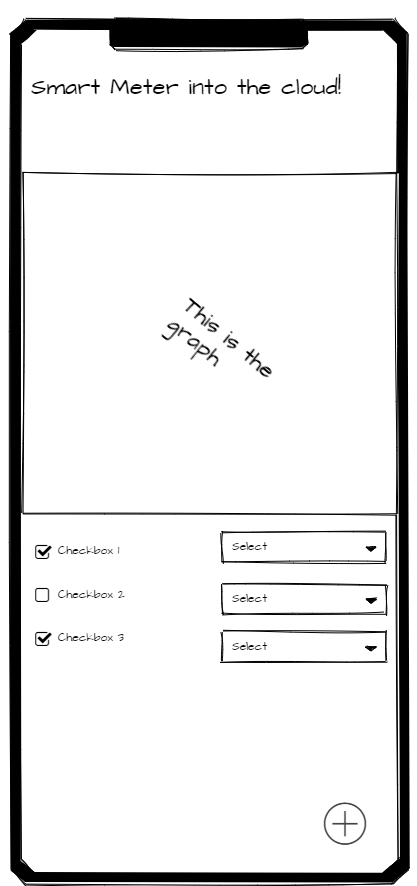
\includegraphics[width=0.5\textwidth]{gfx/entwurf_ui.png}
    \caption{
        Erster Entwurf der Benutzerschnittstelle.
    }
    \label{fig:entwurf_ui}
\end{figure}
Der in Abblidung \ref{fig:entwurf_ui} gezeigte Entwurf einer Benutzerschnittstelle
veranschaulicht grob, wie die einzelnen Komponenten angeordnet werden könnten.
Sie besteht aus zwei Bereichen: Eine Fläche, auf welcher die Messdaten visualisiert werden können.
Diese ist im Entwurf mit ``This is the graph`` beschriftet.
Darunter sind einige Eingabekomponenten angeordnet, welche bspw. dazu dienen können,
zwischen verschiedenen Messdatentypen umzuschalten oder eine benutzerdefinierte Zeitspanne
zu wählen.

Dieser Entwurf deckt somit alle Anforderungen ab, welche in der Aufgabenstellung (Anhang \ref{anhang:aufgabenstellung}) beschrieben wurden.


